%%%%%%%%%%%%%%%%%%%%%%%%%%%%%%%%%%%%%%%%%
% Programming/Coding Assignment
% LaTeX Template
%
% This template has been downloaded from:
% http://www.latextemplates.com
%
% Original author:
% Ted Pavlic (http://www.tedpavlic.com)
%
% Note:
% The \lipsum[#] commands throughout this template generate dummy text
% to fill the template out. These commands should all be removed when 
% writing assignment content.
%
% This template uses a Perl script as an example snippet of code, most other
% languages are also usable. Configure them in the "CODE INCLUSION 
% CONFIGURATION" section.
%
%%%%%%%%%%%%%%%%%%%%%%%%%%%%%%%%%%%%%%%%%

%----------------------------------------------------------------------------------------
%	PACKAGES AND OTHER DOCUMENT CONFIGURATIONS
%----------------------------------------------------------------------------------------



\documentclass{article}

\usepackage{fancyhdr} % Required for custom headers
\usepackage{lastpage} % Required to determine the last page for the footer
\usepackage{extramarks} % Required for headers and footers
\usepackage[usenames,dvipsnames]{color} % Required for custom colors
\usepackage{graphicx} % Required to insert images
\usepackage{listings} % Required for insertion of code
\usepackage{courier} % Required for the courier font
\usepackage{lipsum} % Used for inserting dummy 'Lorem ipsum' text into the template
\usepackage{setspace}
\usepackage{color}
\usepackage{comment}
\usepackage{caption}
\usepackage[T1]{fontenc}
\usepackage{hyperref}
\usepackage{natbib}
\usepackage{underscore}
\usepackage{subfigure}
\usepackage{fixltx2e}
\usepackage{textcomp}

\hypersetup{
    colorlinks=true,
    linkcolor=blue,
    filecolor=magenta,      
    urlcolor=cyan,
    breaklinks=true
}

\usepackage[]{algorithm2e}
\usepackage{pdfpages}
\usepackage{tikz}




%For python inclusion (http://widerin.org/blog/syntax-highlighting-for-python-scripts-in-latex-documents)
\definecolor{Code}{rgb}{0,0,0}
\definecolor{Decorators}{rgb}{0.5,0.5,0.5}
\definecolor{Numbers}{rgb}{0.5,0,0}
\definecolor{MatchingBrackets}{rgb}{0.25,0.5,0.5}
\definecolor{Keywords}{rgb}{0,0,1}
\definecolor{self}{rgb}{0,0,0}
\definecolor{Strings}{rgb}{0,0.63,0}
\definecolor{Comments}{rgb}{0,0.63,1}
\definecolor{Backquotes}{rgb}{0,0,0}
\definecolor{Classname}{rgb}{0,0,0}
\definecolor{FunctionName}{rgb}{0,0,0}
\definecolor{Operators}{rgb}{0,0,0}
\definecolor{Background}{rgb}{0.98,0.98,0.98}

% Margins
\topmargin=-0.45in
\evensidemargin=0in
\oddsidemargin=0in
\textwidth=6.5in
\textheight=9.0in
\headsep=0.25in

\linespread{1.1} % Line spacing

% Set up the header and footer
\pagestyle{fancy}
\lhead{\hmwkAuthorName} % Top left header
\chead{\hmwkClass\ (\hmwkClassInstructor\ \hmwkClassTime): \hmwkTitle} % Top center head
\chead{\hmwkClass\ (\hmwkClassInstructor): \hmwkTitle} % Top center head
\rhead{\firstxmark} % Top right header
\lfoot{\lastxmark} % Bottom left footer
\cfoot{} % Bottom center footer
\rfoot{Page\ \thepage\ of\ \protect\pageref{LastPage}} % Bottom right footer
\renewcommand\headrulewidth{0.4pt} % Size of the header rule
\renewcommand\footrulewidth{0.4pt} % Size of the footer rule

\setlength\parindent{0pt} % Removes all indentation from paragraphs

%----------------------------------------------------------------------------------------
%	CODE INCLUSION CONFIGURATION
%----------------------------------------------------------------------------------------

\definecolor{MyDarkGreen}{rgb}{0.0,0.4,0.0} % This is the color used for comments
\lstloadlanguages{Perl} % Load Perl syntax for listings, for a list of other languages supported see: ftp://ftp.tex.ac.uk/tex-archive/macros/latex/contrib/listings/listings.pdf
\lstset{language=Perl, % Use Perl in this example
        frame=single, % Single frame around code
        basicstyle=\small\ttfamily, % Use small true type font
        keywordstyle=[1]\color{Blue}\bf, % Perl functions bold and blue
        keywordstyle=[2]\color{Purple}, % Perl function arguments purple
        keywordstyle=[3]\color{Blue}\underbar, % Custom functions underlined and blue
        identifierstyle=, % Nothing special about identifiers                                         
        commentstyle=\usefont{T1}{pcr}{m}{sl}\color{MyDarkGreen}\small, % Comments small dark green courier font
        stringstyle=\color{Purple}, % Strings are purple
        showstringspaces=false, % Don't put marks in string spaces
        tabsize=5, % 5 spaces per tab
        %
        % Put standard Perl functions not included in the default language here
        morekeywords={rand},
        %
        % Put Perl function parameters here
        morekeywords=[2]{on, off, interp},
        %
        % Put user defined functions here
        morekeywords=[3]{test},
       	%
        morecomment=[l][\color{Blue}]{...}, % Line continuation (...) like blue comment
        numbers=left, % Line numbers on left
        firstnumber=1, % Line numbers start with line 1
        numberstyle=\tiny\color{Blue}, % Line numbers are blue and small
        stepnumber=5 % Line numbers go in steps of 5
}

% Creates a new command to include a perl script, the first parameter is the filename of the script (without .pl), the second parameter is the caption
\newcommand{\perlscript}[2]{
\begin{itemize}
\item[]\lstinputlisting[caption=#2,label=#1]{#1.pl}
\end{itemize}
}


%----------------------------------------------------------------------------------------
%	DOCUMENT STRUCTURE COMMANDS
%	Skip this unless you know what you're doing
%----------------------------------------------------------------------------------------

% Header and footer for when a page split occurs within a problem environment
\newcommand{\enterProblemHeader}[1]{
\nobreak\extramarks{#1}{#1 continued on next page\ldots}\nobreak
\nobreak\extramarks{#1 (continued)}{#1 continued on next page\ldots}\nobreak
}

% Header and footer for when a page split occurs between problem environments
\newcommand{\exitProblemHeader}[1]{
\nobreak\extramarks{#1 (continued)}{#1 continued on next page\ldots}\nobreak
\nobreak\extramarks{#1}{}\nobreak
}

\setcounter{secnumdepth}{0} % Removes default section numbers
\newcounter{homeworkProblemCounter} % Creates a counter to keep track of the number of problems

\newcommand{\homeworkProblemName}{}
\newenvironment{homeworkProblem}[1][Problem \arabic{homeworkProblemCounter}]{ % Makes a new environment called homeworkProblem which takes 1 argument (custom name) but the default is "Problem #"
\stepcounter{homeworkProblemCounter} % Increase counter for number of problems
\renewcommand{\homeworkProblemName}{#1} % Assign \homeworkProblemName the name of the problem
\section{\homeworkProblemName} % Make a section in the document with the custom problem count
\enterProblemHeader{\homeworkProblemName} % Header and footer within the environment
}{
\exitProblemHeader{\homeworkProblemName} % Header and footer after the environment
}

\newcommand{\problemAnswer}[1]{ % Defines the problem answer command with the content as the only argument
\noindent\framebox[\columnwidth][c]{\begin{minipage}{0.98\columnwidth}#1\end{minipage}} % Makes the box around the problem answer and puts the content inside
}

\newcommand{\homeworkSectionName}{}
\newenvironment{homeworkSection}[1]{ % New environment for sections within homework problems, takes 1 argument - the name of the section
\renewcommand{\homeworkSectionName}{#1} % Assign \homeworkSectionName to the name of the section from the environment argument
\subsection{\homeworkSectionName} % Make a subsection with the custom name of the subsection
\enterProblemHeader{\homeworkProblemName\ [\homeworkSectionName]} % Header and footer within the environment
}{
\enterProblemHeader{\homeworkProblemName} % Header and footer after the environment
}

%----------------------------------------------------------------------------------------
%	NAME AND CLASS SECTION
%----------------------------------------------------------------------------------------

\newcommand{\hmwkTitle}{Homework 7\\ Clustering} % Assignment title
%\newcommand{\hmwkDueDate}{Tuesday,\ February\ 25,\ 2020} % Due date
\newcommand{\hmwkClass}{Web Science} % Course/class
%\newcommand{\hmwkClassTime}{10:30am} % Class/lecture time
\newcommand{\hmwkClassInstructor}{Dr.Michele Weigle} % Teacher/lecturer
\newcommand{\hmwkAuthorName}{Harveen Kaur} % Your name

%----------------------------------------------------------------------------------------
%	TITLE PAGE
%----------------------------------------------------------------------------------------

\title{
\vspace{2in}
\textmd{\textbf{\hmwkClass:\ \hmwkTitle}}\\
%\normalsize\vspace{0.1in}\small{Due\ on\ \hmwkDueDate}\\
%\vspace{0.1in}\large{\textit{\hmwkClassInstructor\ \hmwkClassTime}}
\vspace{0.1in}\large{\textit{\hmwkClassInstructor}}
\vspace{3in}
}

\author{\textbf{\hmwkAuthorName}}
\date{Thursday,April 9,2020} % Insert date here if you want it to appear below your name

%----------------------------------------------------------------------------------------

\begin{document}

\maketitle
\newpage



%----------------------------------------------------------------------------------------
%	TABLE OF CONTENTS
%----------------------------------------------------------------------------------------

%\setcounter{tocdepth}{1} % Uncomment this line if you don't want subsections listed in the ToC

\newpage
\tableofcontents
\newpage

%----------------------------------------------------------------------------------------
%	PROBLEM 1
%----------------------------------------------------------------------------------------

% To have just one problem per page, simply put a \clearpage after each problem

\begin{homeworkProblem}

Generate a list of 100 popular accounts on Twitter. The accounts must be verified, have > 10,000 followers, and have > 5000 tweets. See GET users/lookup and User object for details on obtaining this information for a set of accounts. You may also generate this information manually by visiting individual account pages. For example:\\

\begin{itemize}
\item https://twitter.com/weiglemc - not verified, 414 followers, 2189 tweets - don't include
\item https://twitter.com/WNBA - verified (blue checkmark), 615,000+ followers, 69,000+ tweets - could include
\end{itemize}
Save the list of accounts (screen_names) in a text file (one per line) and upload to your GitHub repo.\\

Download 200 tweets from the 100 accounts. See GET statuses/user_timeline for details. Note that you may receive fewer than 200 tweets in a single API call due to deleted or protected tweets. It's OK as long as you get somewhere close to 200 tweets for each account.\\

Save the responses received from the 100 accounts to your GitHub repo. It can all be in a single file or a separate file for each account. Since this is an intermediate file, the format is up to you.
Find 3 users who are closest to you in terms of age, gender, and occupation.

\\
This user is the substitute you.\\\\
%\problemAnswer{
\textbf{SOLUTION :}\\\\
I collected the information by manually visiting individual account pages. I followed the criteria of the account being verified, having > 10,000 followers and have > 5000 tweets. The list of twitter handles can be found in the file \textbf{twitterHandler}. I used 112 handles to collect data.
 

  
\begin{lstlisting}[language=Python, caption=Assignment7_1.py]
1.YouTube
2.jimmyfallon
3.Google
4.amazon
5.amazonmusic
6.Uber
7.lyft
8.tim_cook
9.BillGates
10.elonmusk
11.richardbranson
12.rupertmurdoch
13.levie
      
\end{lstlisting}
\item\textbf Above given are a few twitter handles that I used. The file \textbf{twitterHandler} is available in the GitHub repo.



\begin{lstlisting}

import twitter
import preprocessor as p
import collections
import re

# For removing URLs from the tweets 
url_regex = 'http[s]?://(?:[a-zA-Z]|[0-9]|[$-_@.&+]|[!*\(\), ]|(?:%[0-9a-fA-F][0-9a-fA
-F]))+'

# for removing  extra emojis
remove_list = ["⭐", "��", "����","��"]

res_dict = collections.defaultdict(lambda: collections.defaultdict(int))

#for removing URLs, Emojis, Smileys and Solo Numbers.
p.set_options(p.OPT.URL, p.OPT.EMOJI, p.OPT.SMILEY, p.OPT.NUMBER)

#user_list = ["sundarpichai", "Android","elonmusk"]
user_list = open('twitterHandler.txt','r').read().split('\n')

'''
Create Twitter Instance. All the fields can be collected from the developer site of
Twitter
I also used the tweet mode as extented to get all the tweet text data in a response 
header.
'''
api = twitter.Api(consumer_key='#################',
                consumer_secret='################',
                access_token_key='################',
                access_token_secret='################',
                sleep_on_rate_limit=True, tweet_mode="extended" 
                )

for user in user_list:
    statuses = api.GetUserTimeline(screen_name=user, count=200)
    texts = [ x.full_text for x in statuses ]
    text = " ".join(texts)
    ntext = re.sub(url_regex, "",  text)
    n2text = p.clean(ntext)
    n3text = n2text
    for x in remove_list:
        n3text = n3text.replace(x, "")
    # n4list = re.split(r'[;,\s()."“]', n3text) 
    # Split words by all non-alpha characters and remove unecesary spaces.
    words = re.compile(r'[^A-Z^a-z]+').split(n3text)
    # Convert to lowercase
    n5list = [word.lower() for word in words if word != '']
    res_dict[user].update(dict(collections.Counter(n5list)))


key_list = set()
for user in list(res_dict.keys()):
    key_list.update(set(res_dict[user].keys()))

key_list = list(key_list)

with open("tweetdata.txt", "w") as f:
    f.write("Username")
    for k in key_list:
        f.write(f"\t{ k }")
    f.write("\n")
    for user in user_list:
        f.write(f"{ user }")
        for k in key_list:
            f.write(f"\t{ res_dict[user][k] }")
        f.write("\n")

\end{lstlisting}
\textbf{}Above given code generates the account term matrix.
%}
\end{homeworkProblem}


%----------------------------------------------------------------------------------------
%   PROBLEM 2
%----------------------------------------------------------------------------------------

\begin{homeworkProblem}
 Generate an account-term matrix from the accounts' tweets.\\

Using the responses from Q1, extract the text from each tweet to generate terms. Remove any URIs in the tweets, but keep regular text and hashtags as terms. Limit the number of terms to the most "popular" (i.e., frequent) 1000 terms, this is after the criteria on p. 32 (chapter 3 PCI book) (slide 11 - Week 10) has been satisfied.\\

Save the terms for each account in a file and upload to your GitHub repo. It can all be in a single file or a separate file for each account. Since this is an intermediate file, the format is up to you.\\

In the account-term matrix, the account screen_name is the account identifier and should be start each row of the matrix. Use the (max 1000) terms for the columns of the matrix. The values are the frequency of occurrence. Essentially you are replicating the format of the "blogdata.txt" file included with the PCI book code.\\

Save the matrix in a text file (either tab-separated like blogdata.txt or comma-separated) and upload to your GitHub repo.\\\\
%\problemAnswer{
 \textbf{SOLUTION}\\\\
Account term matrix was created using the code given in listing7_1. The account term matrix was generated using the tweets from 112 accounts(verified).
 
\begin{lstlisting}[language=Python, caption=Assignment7_2.py]
with open("tweetdata.txt", "w") as f:
    f.write("Username")
    for k in key_list:
        f.write(f"\t{ k }")
    f.write("\n")
    for user in user_list:
        f.write(f"{ user }")
        for k in key_list:
            f.write(f"\t{ res_dict[user][k] }")
        f.write("\n")
\end{lstlisting}
\textbf{}The result is stored in the file tweetdata.txt and is available on GitHub.

%}
\end{homeworkProblem}
\clearpage
\newpage

%----------------------------------------------------------------------------------------
%   PROBLEM 3
%----------------------------------------------------------------------------------------

\begin{homeworkProblem}
Create an ASCII dendrogram and a JPEG dendrogram that uses hierarchical clustering to cluster the most similar accounts (see slides 21 & 23 - Week 10). Include the JPEG in your report and upload the ASCII file to GitHub (it will be too unwieldy for inclusion in the report).\\
\end{itemize}
%\problemAnswer{
 \textbf{SOLUTION}\\

The python script denodo.py calls the methods from clusters. \\
Using the file \textbf{tweetdata.txt} we get the ASCII dendrogram and the JPEG dendrogram.\\
Reference: Slide 21 and 23.
 
\begin{lstlisting}[language=Python, caption=Assignment7_3.py]
import clusters
import sys


def createDendrogram():
    Username, colnames, data = clusters.readfile('tweetdata.txt')
    cluster = clusters.hcluster(data)
    clusters.drawdendrogram(cluster, Username, jpeg='Dendrogram.jpg')
    f = open("ASCII.txt", 'w')
    sys.stdout = f
    clusters.printclust(cluster, labels=Username)
    f.close()
    sys.stderr.close()


if __name__ == "__main__":
    createDendrogram()
\end{lstlisting}

\item\textbf{}The diagram given below displays the generated JPEG dendogram. The ASCII dendrogram is available on GitHub. I have not uploaded it here as it is to unwieldy to be included in the report(as mentioned in the problem). 


\newpage
\begin{figure}[h]
  \centering
    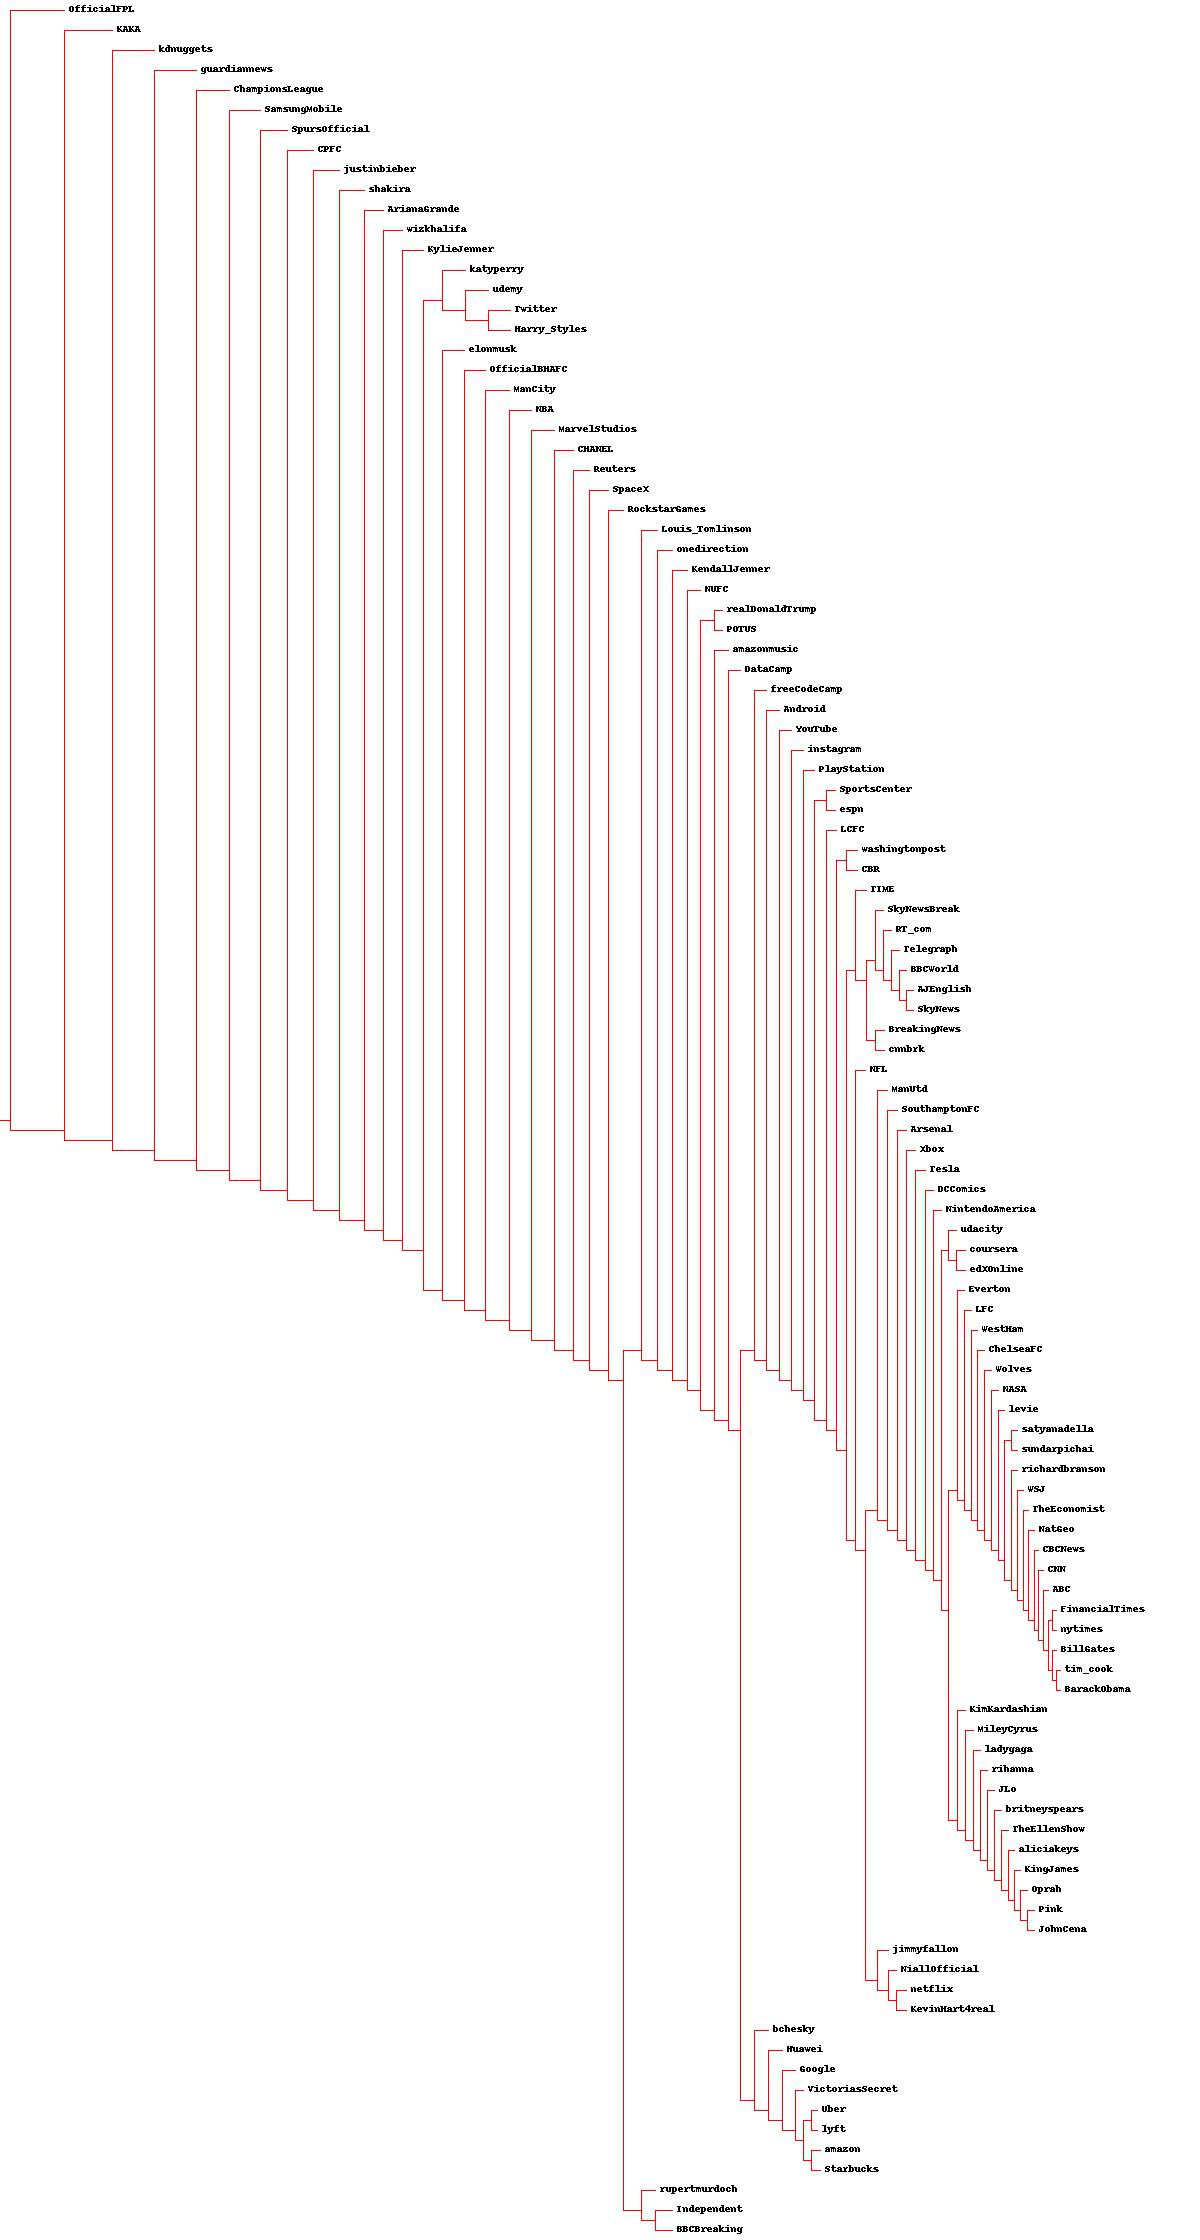
\includegraphics[width=0.7\textwidth]{Dendrogram.jpg}
      \caption{JPEG dendrogram }
\end{figure}

\end{homeworkProblem}
\clearpage
\newpage
%----------------------------------------------------------------------------------------
%   PROBLEM 4
%----------------------------------------------------------------------------------------

\begin{homeworkProblem}
Cluster the accounts using k-Means, using k=5,10,20 (see slide 37 - Week 10). Print the accounts in each cluster, for each value of k. How many iterations were required for each value of k?\\

\textbf{SOLUTION}\\
\textbf{}With the help of the code given in the slide 37 I coded the script kmeanclustering.py.

\begin{lstlisting}[language=Python, caption=Assignment7_4.py]
import clusters
def kMean():
    kMeanValues = [5, 10, 20]
    Username, colnames, data = clusters.readfile('tweetdata.txt')
    for i in kMeanValues:

        kclust, itercount = clusters.kcluster(data, k=i)
        print(kclust)
        f = open("kclust_%d.txt" % i, 'w')
        f.write("Total Number Of Iterations: %d \n" % itercount)
        print(len(kclust))
        clusterCount = 1
        for cluster in kclust:
            i=1
            f.write("---\n")
            f.write("Cluster %d \n" % clusterCount)
            for tweetID in cluster:
                f.write(str(i)+".\t"+Username[tweetID] + "\n")
                i+=1
            f.write("\n")
            clusterCount+=1
if __name__ == "__main__":
    kMean()
\end{lstlisting}
The results have been uploaded as text files \textbf{kclust_5}, \textbf{kclust_10} and \textbf{kclust_20} respectively.For the clusters it took 6 iterations, 5 iterations and 5 iterations respectively.\\\\

\end{homeworkProblem}

%----------------------------------------------------------------------------------------
%   PROBLEM 5
%----------------------------------------------------------------------------------------

\begin{homeworkProblem}
 Use MDS to create a JPEG of the accounts (see slide 50 - Week 10). Include the JPEG in your report. How many iterations were required?\\

\textbf{SOLUTION}\\
 
\textbf{}Created the following python script.

\begin{lstlisting}[language=Python, caption=Assignment7_5.py]
import clusters    


Username, words, data = clusters.readfile('tweetdata.txt')
coords, itercount = clusters.scaledown(data)
clusters.draw2d(coords, labels=Username, jpeg='mds.jpg')
print ('Iteration count: %d' % itercount)

\end{lstlisting}
\textbf{}To generate the result 1 iteration was required.
\begin{figure}[h]
  \centering
    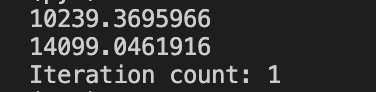
\includegraphics[width=0.5\textwidth]{mdsiteration.png}
      \caption{MDS iteration}
\end{figure}
\begin{figure}[h]
  \centering
    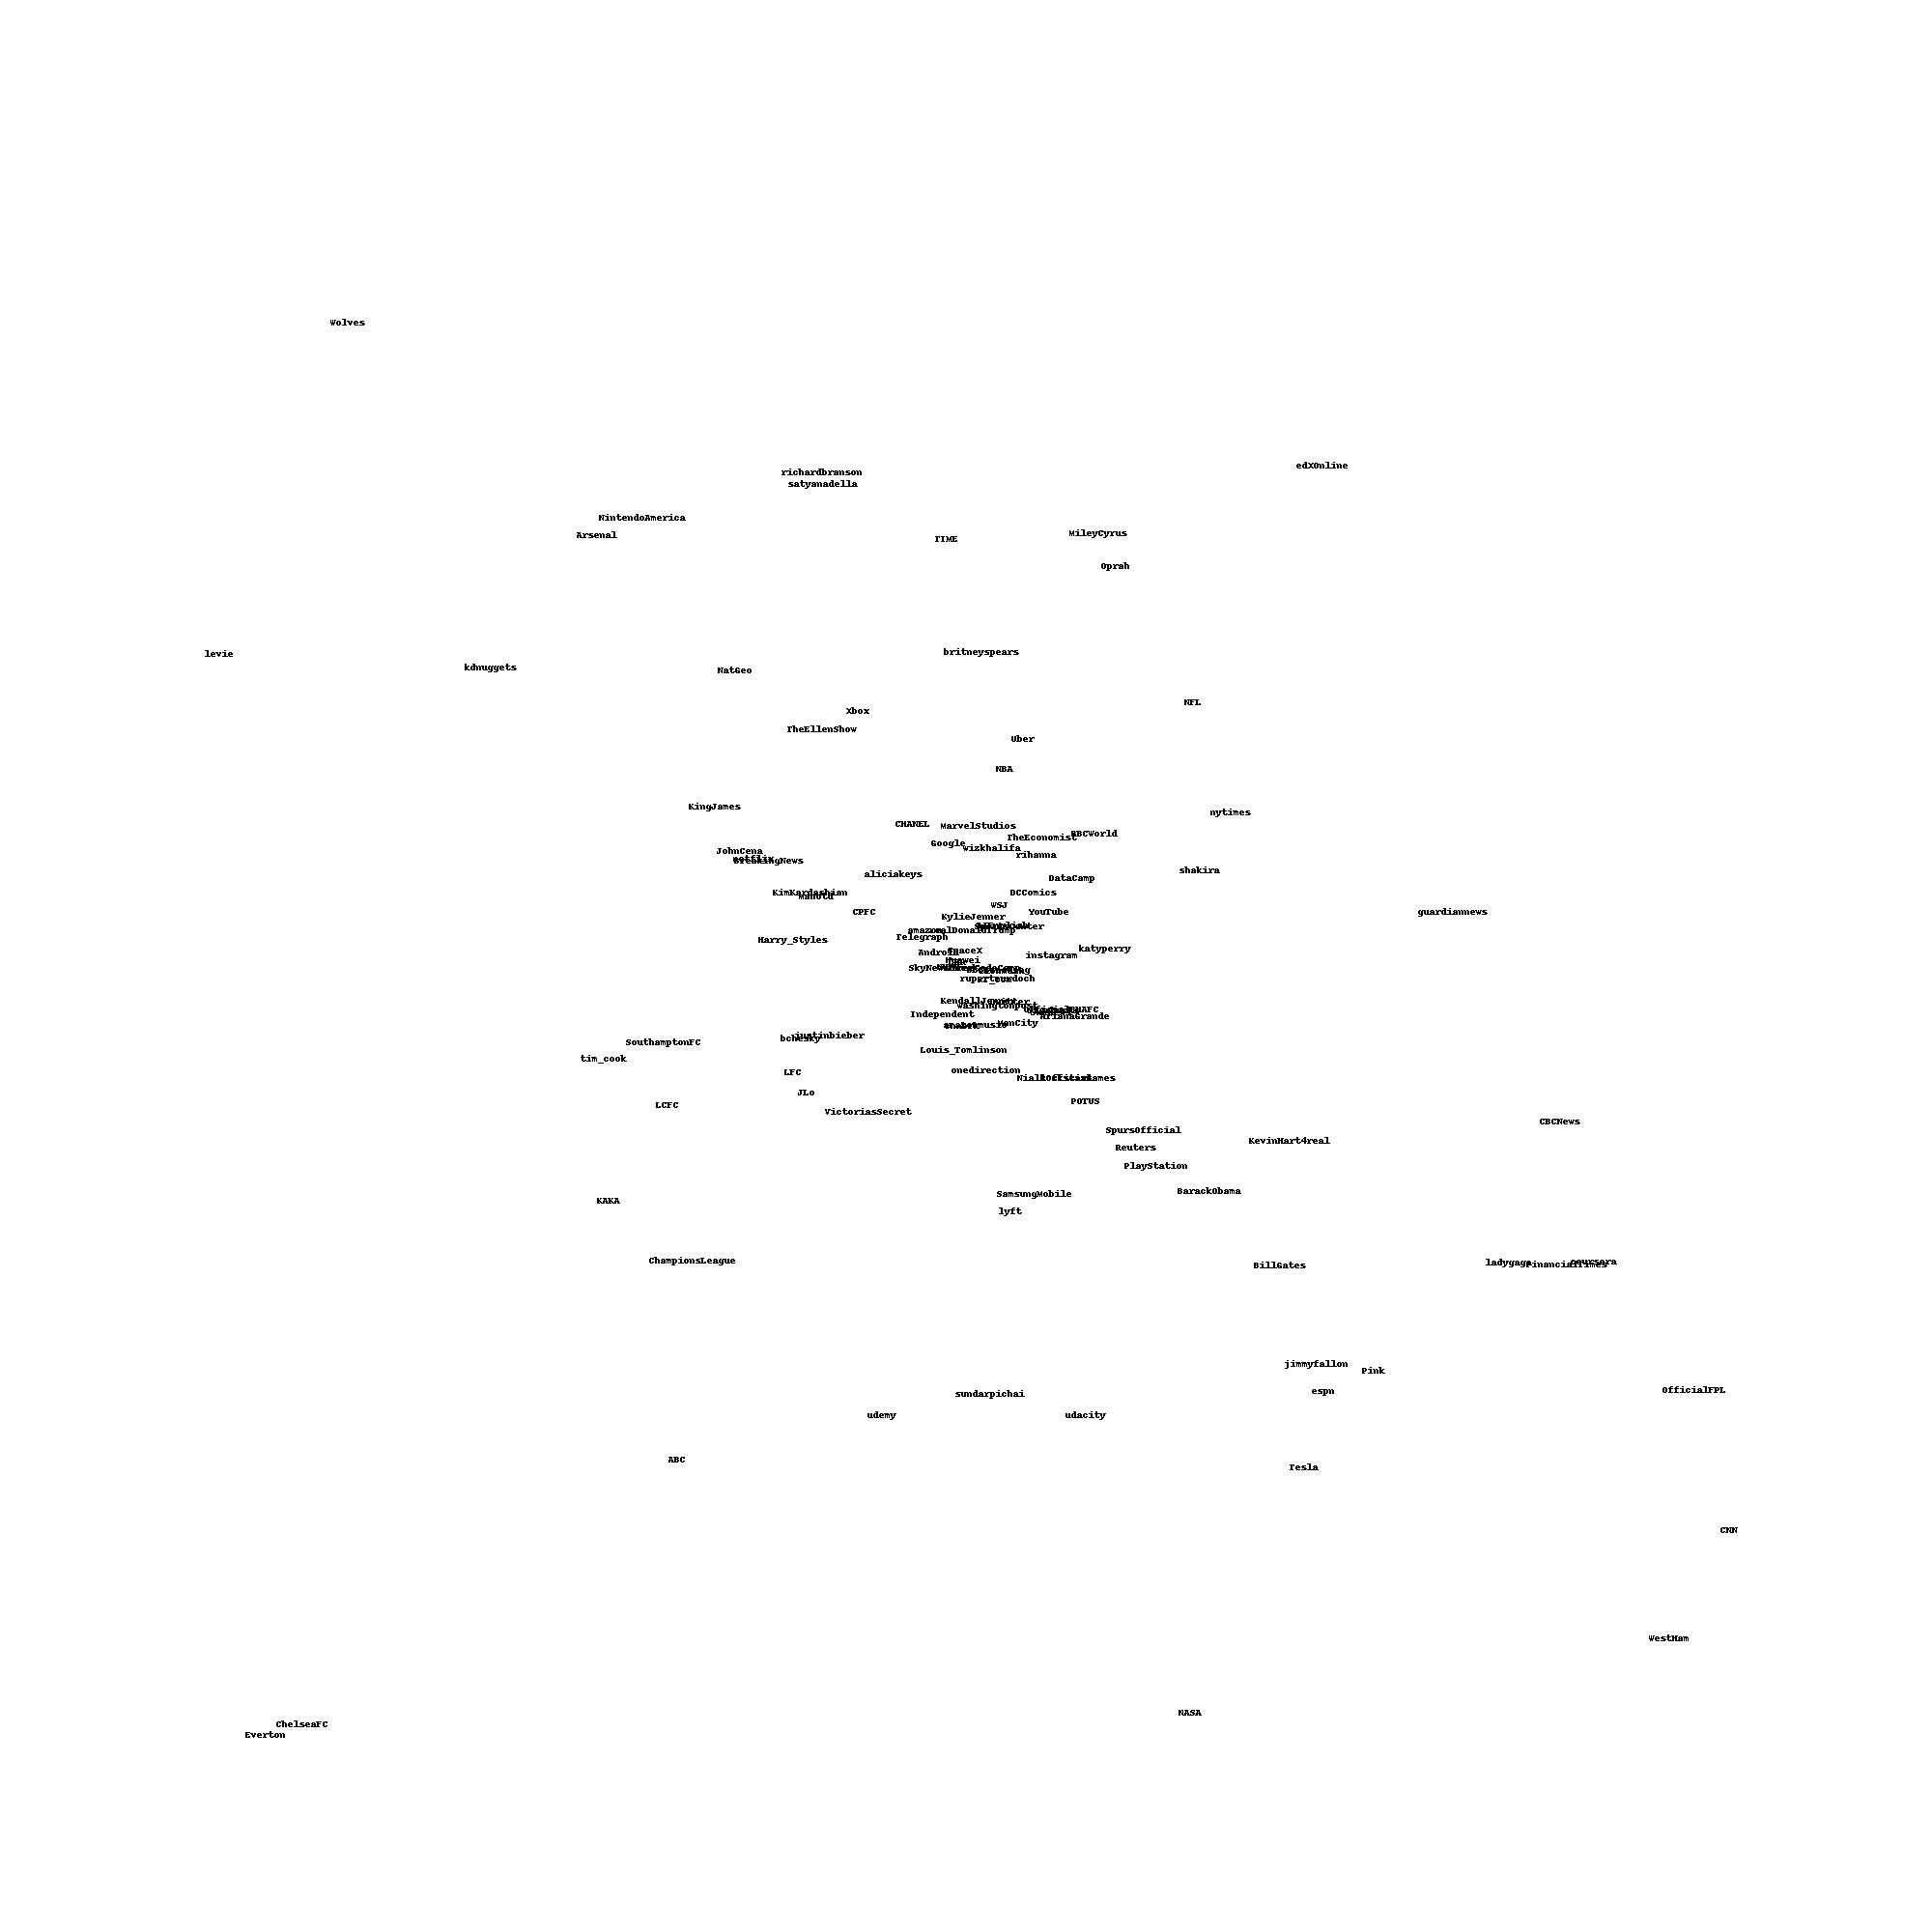
\includegraphics[width=1.1\textwidth]{mds.jpg}
      \caption{MDS}
\end{figure}

\end{homeworkProblem}



\bibliographystyle{plain}
\bibliography{A1bibFile}

\end{document}
